% =============================================================================
% SECCIÓN 2.4: ALMACENAMIENTO DISTRIBUIDO: IPFS
% =============================================================================

\section{IPFS}
\label{sec:ipfs}

El InterPlanetary File System (IPFS) es un protocolo peer-to-peer de sistema de archivos distribuido diseñado para conectar todos los dispositivos de cómputo con el mismo sistema de archivos, utilizando direccionamiento basado en contenido (content-addressing) en lugar de ubicación (location-addressing como HTTP) \cite{benet2014ipfs}. Esta arquitectura fundamental permite la distribución descentralizada de datos, la deduplicación automática y la verificación criptográfica de integridad, posicionando a IPFS como una solución complementaria a blockchains y BlockDAG para el almacenamiento de grandes volúmenes de datos con trazabilidad verificable.

\subsubsection{Arquitectura IPFS: Sistema de Archivos Distribuido}

IPFS está estructurado como una pila de sub-protocolos modulares e intercambiables, organizados en siete capas funcionales que proporcionan identidad, enrutamiento, intercambio de bloques y versionado de contenido \cite{benet2014ipfs}. La capa de Identidades genera y verifica la identidad de nodos mediante NodeId = hash(PublicKey), siguiendo el esquema de identidad basado en PKI descrito en la especificación de arquitectura IPFS \cite{benet2014ipfs,ipfs_architecture}. Este esquema utiliza criptografía S/Kademlia para resistencia a ataques Sybil, donde los nodos son identificados por un NodeId que corresponde al hash criptográfico de una clave pública, creado mediante el puzzle criptográfico estático de S/Kademlia \cite{benet2014ipfs}. La capa de Red soporta múltiples protocolos de transporte (WebRTC, uTP/LEDBAT) con traversal de NAT mediante ICE y direccionamiento multiaddr agnóstico a la capa de transporte.

La capa de Routing implementa una Tabla de Hash Distribuida (DHT) basada en S/Kademlia y Coral DSHT \cite{benet2014ipfs,freedman2004coral,blockchainMeetsDFS}. Coral DSHT extiende Kademlia de tres formas particularmente importantes: organiza una jerarquía de DSHTs separadas llamadas clusters dependiendo de la región y tamaño, optimiza la latencia mediante una infraestructura de indexación jerárquica, y utiliza una abstracción denominada Distributed Sloppy Hash Table (DSHT) \cite{freedman2004coral,benet2014ipfs}. IPFS logra esto utilizando una DSHT basada en S/Kademlia y Coral, almacenando valores pequeños directamente y valores grandes como referencias (provider records) \cite{benet2014ipfs,blockchainMeetsDFS}. El protocolo de Intercambio (BitSwap) permite que los nodos intercambien bloques mediante un sistema de crédito/débito y estrategias de envío probabilísticas que incentivan la distribución de contenido y resisten comportamientos de nodos que solo consumen sin compartir, inspirado conceptualmente en BitTorrent.

La capa de Objetos implementa un Grafo Acíclico Dirigido (Merkle DAG) donde cada objeto contiene enlaces y datos, donde los enlaces son hashes criptográficos de los objetos destino. La capa de Archivos proporciona un modelo de objetos versionado similar a Git, con tipos blob (datos brutos), list (secuencias de bloques para deduplicación), tree (directorios) y commit (snapshots de historial). Finalmente, la capa de Nombres (IPNS) ofrece un sistema de nombres mutable auto-certificado usando criptografía de clave pública para mapear NodeId a CIDs mutables.

Filosóficamente, IPFS puede visualizarse como un único swarm de BitTorrent intercambiando objetos dentro de un solo repositorio Git" \cite{benet2014ipfs}, combinando DHT (Kademlia), intercambio de bloques (BitTorrent), versionado (Git) y auto-certificación (SFS). Esta arquitectura proporciona propiedades clave: content addressing (cada objeto identificado por su checksum multihash), resistencia a alteraciones (verificación mediante checksum), y deduplicación automática (objetos con contenido idéntico comparten el mismo hash y se almacenan una sola vez).

La Figura~\ref{fig:ipfs_stack} ilustra la arquitectura de pila de IPFS con sus siete capas funcionales, mostrando la organización jerárquica desde la capa de aplicación hasta la capa de red.

\begin{figure}[htbp]
    \centering
    \shorthandoff{>}
    \begin{tikzpicture}[
        layer/.style={
            rectangle,
            draw,
            fill=blue!20,
            text width=5cm,
            text centered,
            rounded corners,
            minimum height=1cm
        },
        arrow/.style={->, thick, >=stealth},
        node distance=0.6cm
    ]
    
    \node[layer] (nombres) {7. Nombres (IPNS)};
    \node[layer, below=of nombres] (archivos) {6. Archivos (Git-like)};
    \node[layer, below=of archivos] (objetos) {5. Objetos (Merkle DAG)};
    \node[layer, below=of objetos] (bitswap) {4. Intercambio (BitSwap)};
    \node[layer, below=of bitswap] (routing) {3. Routing (DHT)};
    \node[layer, below=of routing] (red) {2. Red (Multi-protocol)};
    \node[layer, below=of red] (identidades) {1. Identidades (S/Kademlia)};
    
    \draw[arrow] (identidades) -- (red);
    \draw[arrow] (red) -- (routing);
    \draw[arrow] (routing) -- (bitswap);
    \draw[arrow] (bitswap) -- (objetos);
    \draw[arrow] (objetos) -- (archivos);
    \draw[arrow] (archivos) -- (nombres);
    
    \end{tikzpicture}
    \shorthandon{>}
    \caption{Arquitectura de pila de IPFS con sus siete capas funcionales.}
    \label{fig:ipfs_stack}
\end{figure}


    

\subsubsection{Content Identifiers (CIDs): Estructura y Hash Criptográfico}

Un Content Identifier (CID) es un identificador auto-descriptivo que contiene tanto el codec (formato de interpretación de datos) como un multihash (hash auto-descriptivo que especifica la función hash utilizada) \cite{benet2014ipfs}. La estructura de multihash sigue el formato $\langle function\_code \rangle \langle digest\_length \rangle \langle digest\_bytes \rangle$, donde function\_code identifica el algoritmo hash (ej. SHA-256, BLAKE3), digest\_length especifica la longitud del hash en bytes, y digest\_bytes contiene el hash criptográfico en sí.

IPFS soporta dos versiones de CID. CIDv0 (legacy) utiliza un formato simplificado donde el multihash se codifica en Base58, produciendo identificadores de 46 caracteres que comienzan con "Qm". CIDv1 (moderno) emplea un formato extensible con prefijos explícitos: $\langle multibase\_prefix \rangle \langle cid\_version \rangle \langle multicodec \rangle \langle multihash \rangle$, donde multibase\_prefix indica la codificación base utilizada (ej. base32, base58btc), cid\_version especifica la versión del CID, multicodec identifica el formato del contenido objetivo (dag-pb/UnixFS, dag-cbor, raw), y multihash contiene el hash del contenido.

Las propiedades fundamentales de los CIDs incluyen determinismo (el mismo contenido produce el mismo CID en cualquier nodo), inmutabilidad (cualquier modificación genera un CID diferente), y forward-compatibility (CIDv1 permite evolucionar algoritmos hash y codecs sin romper compatibilidad). Para archivos grandes, IPFS los divide en chunks, donde el CID corresponde al hash del bloque raíz del DAG, no del archivo completo, permitiendo chunking flexible, deduplicación y Merkle trees balanceados. Los CIDs se utilizan en URIs de la forma /ipfs/$\langle$CID$\rangle$/$\langle$path$\rangle$, donde IPFS resuelve el path recorriendo el Merkle DAG desde el hash raíz y navegando por links nombrados.

La Figura~\ref{fig:cid_resolution} muestra el flujo de resolución de un CID, desde la petición del usuario hasta la reconstrucción del contenido mediante DHT y BitSwap.

\begin{figure}[htbp]
\centering
\shorthandoff{>}
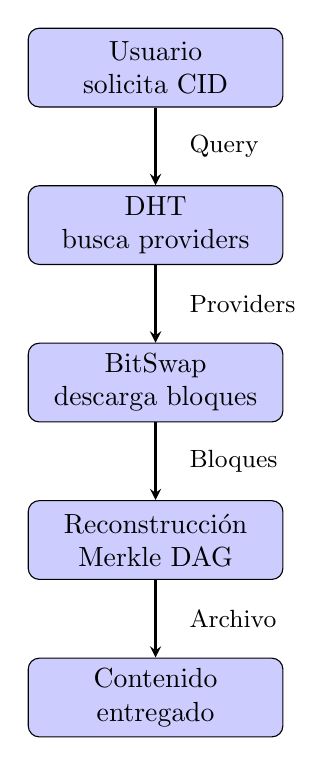
\begin{tikzpicture}[
    node/.style={rectangle, draw, fill=blue!20, text width=3cm, text centered, rounded corners, minimum height=1cm},
    arrow/.style={->,thick,>=stealth}
]
    \node[node] (usuario) at (0,5) {Usuario \\ solicita CID};
    \node[node] (dht) at (0,3) {DHT \\ busca providers};
    \node[node] (bitswap) at (0,1) {BitSwap \\ descarga bloques};
    \node[node] (reconstruccion) at (0,-1) {Reconstrucción \\ Merkle DAG};
    \node[node] (contenido) at (0,-3) {Contenido \\ entregado};
    
    % Flechas con coordenadas intermedias para posicionar etiquetas
    \draw[arrow] (usuario.south) -- node[right, xshift=0.3cm, pos=0.5] {\small Query} (dht.north);
    \draw[arrow] (dht.south) -- node[right, xshift=0.3cm, pos=0.5] {\small Providers} (bitswap.north);
    \draw[arrow] (bitswap.south) -- node[right, xshift=0.3cm, pos=0.5] {\small Bloques} (reconstruccion.north);
    \draw[arrow] (reconstruccion.south) -- node[right, xshift=0.3cm, pos=0.5] {\small Archivo} (contenido.north);
\end{tikzpicture}
\shorthandon{>}
\caption{Flujo de resolución de CID en IPFS: desde la solicitud del usuario hasta la entrega del contenido.}
\label{fig:cid_resolution}
\end{figure}

\subsubsection{Pinning y Gateways: Persistencia y Acceso}

Los nodos IPFS cachean contenido descargado en almacenamiento local, pero este es finito. Un proceso de garbage collection periódico elimina bloques no referenciados para liberar espacio. El pinning (anclaje) marca objetos y sus bloques para que no sean eliminados durante la garbage collection, garantizando persistencia local indefinida \cite{benet2014ipfs}. El pinning recursivo ancla un objeto raíz y todos sus descendientes recursivamente, preservando estructuras completas como árboles de archivos y DAGs versionados.

Los servicios de pinning (pinning services) son terceros que ejecutan nodos IPFS dedicados para anclar datos de usuarios a cambio de una tarifa, asegurando alta disponibilidad y redundancia geográfica. Esta infraestructura es crítica para aplicaciones que requieren garantías de persistencia sin mantener infraestructura propia. Sin embargo, el pinning requiere que al menos un nodo mantenga el contenido vivo; si todos los nodos eliminan el contenido (unpinning), este puede volverse irrecuperable.

Los IPFS Gateways son servidores HTTP que exponen contenido IPFS a navegadores web tradicionales sin requerir que el usuario ejecute un nodo IPFS completo. El funcionamiento típico implica: recepción de petición HTTP en la forma https://$\langle$gateway\_url$\rangle$/ipfs/$\langle$CID$\rangle$/path, resolución del CID mediante DHT para encontrar providers (nodos que tienen el contenido), recuperación de contenido conectando a providers vía Bitswap/Graphsync, descarga de bloques del Merkle DAG y reconstrucción del archivo, y entrega HTTP estándar al navegador del usuario.

Los gateways públicos (ej. ipfs.io, dweb.link) proporcionan acceso conveniente pero introducen puntos de confianza y posible congestión. Los gateways privados/dedicados, ejecutados por organizaciones dentro de su red privada, ofrecen acceso controlado con código confiable. Los subdomain gateways (https://$\langle$CID$\rangle$.ipfs.$\langle$gateway\_url$\rangle$/path) mejoran seguridad cross-origin (CORS) aislando cada CID en su propio subdominio. Los gateways simplifican el acceso (no requieren software especial), proporcionan puente entre HTTP e IPFS ($\leftrightarrow$), y el cacheo inteligente reduce latencia y uso de ancho de banda, aunque introducen limitaciones de confianza donde gateways públicos pueden censurar contenido o registrar actividad.

\subsubsection{Integración con Blockchain y BlockDAG: Off-Chain Storage y On-Chain Metadata}

El almacenamiento de datos grandes on-chain en blockchains tradicionales es costoso (gas fees altos), ineficiente (ledger inflado) y no escalable, dado que blockchains como Ethereum tienen límites de throughput (~15-30 TPS) y tamaño de bloque restringido \cite{yang2023interaction, vasughi2023offchain}. La arquitectura híbrida combina almacenamiento off-chain en IPFS (para datos grandes como archivos, imágenes, videos, datasets) con registro on-chain de metadatos (solo el CID y metadatos críticos como propietario, timestamp, permisos) en blockchain o BlockDAG, manteniendo el ledger ligero y económico \cite{yang2023interaction, haque2024integrated}.

El mecanismo de interacción estándar sigue el siguiente patrón: (1) Carga de datos: el usuario sube un archivo a IPFS (vía nodo local o pinning service), y IPFS devuelve el CID del contenido; (2) Registro on-chain: un smart contract almacena el CID en la blockchain junto con metadatos de propiedad/acceso; (3) Verificación: el CID on-chain actúa como "prueba de existencia" inmutable, donde cualquier modificación del archivo off-chain generaría un CID diferente, detectándose la manipulación; (4) Recuperación: el usuario lee el CID desde la blockchain, luego descarga el contenido desde IPFS usando ese CID (vía gateway o nodo local).

La Figura~\ref{fig:hybrid_architecture} ilustra la arquitectura híbrida Blockchain-IPFS, mostrando el flujo completo desde la carga de datos hasta la recuperación verificable.

\begin{figure}[htbp]
\centering
\shorthandoff{>}
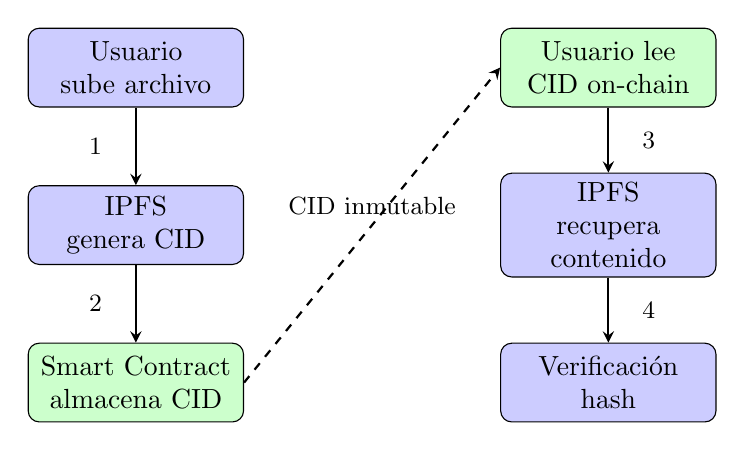
\begin{tikzpicture}[
    box/.style={rectangle, draw, fill=blue!20, text width=2.5cm, text centered, rounded corners, minimum height=1cm},
    blockchain/.style={rectangle, draw, fill=green!20, text width=2.5cm, text centered, rounded corners, minimum height=1cm},
    arrow/.style={->,thick,>=stealth}
]
    % Upload flow
    \node[box] (upload) at (-3,4) {Usuario \\ sube archivo};
    \node[box] (ipfs) at (-3,2) {IPFS \\ genera CID};
    \node[blockchain] (contract) at (-3,0) {Smart Contract \\ almacena CID};
    
    % Retrieval flow
    \node[blockchain] (read) at (3,4) {Usuario lee \\ CID on-chain};
    \node[box] (ipfs2) at (3,2) {IPFS \\ recupera contenido};
    \node[box] (verify) at (3,0) {Verificación \\ hash};
    
    % Arrows upload con etiquetas cerca de las flechas
    \draw[arrow] (upload.south) -- node[left, xshift=-0.3cm, pos=0.5] {\small 1} (ipfs.north);
    \draw[arrow] (ipfs.south) -- node[left, xshift=-0.3cm, pos=0.5] {\small 2} (contract.north);
    
    % Arrows retrieval con etiquetas cerca de las flechas
    \draw[arrow] (read.south) -- node[right, xshift=0.3cm, pos=0.5] {\small 3} (ipfs2.north);
    \draw[arrow] (ipfs2.south) -- node[right, xshift=0.3cm, pos=0.5] {\small 4} (verify.north);
    
    % Connection between upload and retrieval
    \draw[arrow, dashed] (contract.east) -- node[above] {\small CID inmutable} (read.west);
\end{tikzpicture}
\shorthandon{>}
\caption{Arquitectura híbrida Blockchain-IPFS: flujo de carga (izquierda) y recuperación (derecha) con verificación criptográfica.}
\label{fig:hybrid_architecture}
\end{figure}

Esta integración ha sido documentada en múltiples casos de uso: NFTs (Non-Fungible Tokens) almacenan metadatos y arte digital en IPFS con CID referenciado en tokenURI de contratos ERC-721/ERC-1155, garantizando que el asset del NFT sea permanente y verificable; sistemas de Healthcare IoMT almacenan datos encriptados en clusters IPFS mientras smart contracts registran hashes para trazabilidad y privacidad \cite{kumar2020healthcare}; verificación de documentos (diplomas, certificados) almacenados como archivos IPFS con blockchain manteniendo registro de autenticidad.

Los beneficios de la integración incluyen escalabilidad (reducción drástica del tamaño de transacciones on-chain, con ratios de compresión reportados de ~0.0817) \cite{zheng2018blockchain}, reducción de costos (gas fees reducidos al almacenar solo hashes de 32-46 bytes vs. archivos completos), integridad (content-addressing de IPFS + inmutabilidad de blockchain proporcionan prueba criptográfica end-to-end), disponibilidad (IPFS distribuye réplicas vía BitSwap mientras blockchain asegura que el pointer CID sea permanente y resistente a censura), y deduplicación global (múltiples transacciones blockchain pueden referenciar el mismo CID IPFS sin duplicar almacenamiento).

Las limitaciones y consideraciones incluyen dependencia de pinning (si nadie ancla el contenido IPFS, puede volverse inaccesible aunque el CID esté on-chain, mitigado mediante incentivos económicos como Filecoin o SLAs con pinning services), latencia de recuperación (acceso a contenido IPFS puede ser más lento que almacenamiento centralizado debido a DHT lookup + block retrieval, mitigado mediante gateways con CDN), y asunciones de confianza (gateways públicos introducen puntos de confianza, requiriendo nodos locales o gateways privados para operaciones más trustless).

Esta arquitectura híbrida es particularmente relevante para sistemas de monitoreo urbano que requieren almacenamiento frecuente de reportes de tráfico, configuraciones optimizadas y métricas históricas, donde la combinación de IPFS (alto throughput, deduplicación) y BlockDAG (baja latencia, costos reducidos) proporciona una solución escalable y económicamente viable para trazabilidad verificable en entornos de smart cities.

